\chapter{Geodäten, gleichförmige Beschleunigung und der Newtonsche Grenzfall}

Das unmittelbare Problem ist die Gravitation. Genauer gesagt suchen wir die Raumzeitmetrik, die ein nahezu gleichförmiges Gravitationsfeld beschreibt, etwa das Feld in einem kleinen Labor nahe der Erdoberfläche. Der kürzeste Weg zu dieser Metrik ist überraschenderweise kein direkter. Zunächst müssen wir drei geometrische Begriffe operational fassen: kovariante Ableitung, Paralleltransport und geodätische Bewegung.

Diese Begriffe hängen voneinander ab. Die kovariante Ableitung gibt an, wie wir Vektoren an benachbarten Punkten vergleichen. Der Paralleltransport beschreibt, wie wir einen Vektor mitführen, ohne ihn zu drehen. Eine Geodäte erhält man, wenn der mitgeführte Vektor die Tangente an den Weg selbst ist. Liegt der Weg in der Raumzeit statt im Raum, wird dieselbe Geodätengleichung zur Bewegungsgleichung eines frei fallenden Teilchens.

In der zweiten Hälfte der Vorlesung folgt dann ein bemerkenswerter Schritt. Wir bleiben in der flachen Minkowski-Raumzeit, beschreiben sie aber mit Koordinaten, die an eine starr beschleunigte Beobachterfamilie angepasst sind. In diesen Koordinaten sieht die Metrik gravitationsartig aus. In der Nähe eines Beobachters reproduziert sie das Potential eines gleichförmigen Feldes, und ihre Geodäten erfüllen die Newtonsche Gleichung
\begin{equation}
\frac{d^2y}{d\tau^2}=-g.
\end{equation}
Dies ist das Äquivalenzprinzip, als Rechnung formuliert.

\section{Rückblick auf die kovariante Ableitung}

An einem gewählten Punkt \(P\) lassen sich Koordinaten wählen, die möglichst kartesisch sind. Zunächst verwendet die Vorlesung den Ausdruck Gaußsche Normalkoordinaten und schränkt ihn gleich darauf ein. Wichtiger als die Bezeichnung sind die lokalen Bedingungen:
\begin{equation}
g_{mn}(P)=\delta_{mn},
\qquad
\partial_r g_{mn}(P)=0.
\label{eq:l4-normal-point}
\end{equation}
Dies sind Normalkoordinaten an einem einzelnen Punkt. In einer endlichen Umgebung müssen sie nicht kartesisch bleiben. Außerdem gibt es viele solche Bezugssysteme, da ihre Achsen gedreht werden können.

Die Metrik ist mit dem Ableitungsoperator verträglich:
\begin{equation}
\nabla_r g_{mn}=0,
\qquad
\nabla_r g^{mn}=0.
\label{eq:l4-metric-compatibility}
\end{equation}
Für einen Kovektor \(V_s\) lautet die kovariante Ableitung
\begin{equation}
\nabla_r V_s
=
\partial_r V_s-\Gamma^p{}_{rs}V_p.
\label{eq:l4-covector-derivative}
\end{equation}
Die Koeffizienten der Verbindung sind
\begin{equation}
\Gamma^p{}_{rs}
=
\frac{1}{2}g^{pn}
\left(
\partial_s g_{nr}
+\partial_r g_{ns}
-\partial_n g_{rs}
\right).
\label{eq:l4-christoffel}
\end{equation}
Während dieser Ausdruck an der Tafel hergeleitet wird, werden mehrere Indizes korrigiert. Gleichung \eqref{eq:l4-christoffel} ist die vervollständigte Beziehung. Sie ist symmetrisch in \(r\) und \(s\), wie es für die torsionsfreie Levi-Civita-Verbindung zu erwarten ist.

\begin{figure}[htbp]
\centering
\includegraphics[width=0.92\textwidth]{lecture_04_figure_01.png}
\caption{Die Kovektor-Ableitung und die vervollständigte Formel für die Christoffel-Symbole.}
\end{figure}

Da die Christoffel-Symbole aus ersten Ableitungen der Metrik gebildet werden, verschwinden sie bei \(P\) in den Koordinaten \eqref{eq:l4-normal-point}. Sie verschwinden jedoch nicht in jedem Koordinatensystem, selbst wenn der zugrunde liegende Raum flach ist. Daher ist \(\Gamma^p{}_{rs}\) kein Tensor. Genau dieser nicht-tensorielle Charakter ermöglicht es später einem beschleunigten Beobachter, eine Gravitationskraft zu beschreiben, die ein Inertialbeobachter nicht wahrnimmt.

\subsection{Anheben des Vektorindex}

Die entsprechende Ableitung eines Vektors wird nicht als eigenständige Merkregel eingeführt. Sie folgt aus der Metrik. Wir beginnen mit
\begin{equation}
V^n=g^{np}V_p.
\end{equation}
Dann gilt
\begin{align}
\nabla_m V^n
&=\nabla_m\!\left(g^{np}V_p\right) \\
&=(\nabla_m g^{np})V_p+g^{np}\nabla_m V_p \\
&=g^{np}\left(\partial_mV_p-\Gamma^r{}_{mp}V_r\right),
\end{align}
wobei die Metrikverträglichkeit den ersten Term zum Verschwinden bringt. Nach Umordnung der Indizes ergibt sich
\begin{equation}
\nabla_m V^n
=
\partial_m V^n+\Gamma^n{}_{mr}V^r.
\label{eq:l4-vector-derivative}
\end{equation}

\begin{figure}[htbp]
\centering
\includegraphics[width=0.90\textwidth]{lecture_04_figure_02.png}
\caption{Anheben des Index mit der inversen Metrik vor der Ableitung.}
\end{figure}

\begin{figure}[htbp]
\centering
\includegraphics[width=0.90\textwidth]{lecture_04_figure_03.png}
\caption{Die Ableitung mit oberem Index ergibt sich aus der Metrikverträglichkeit und der Produktregel.}
\end{figure}

Die Indexregeln sind also einfach:
\begin{equation}
\boxed{
\begin{aligned}
\text{lower index:}&\quad -\Gamma,\\
\text{upper index:}&\quad +\Gamma.
\end{aligned}}
\end{equation}
Bei einem Tensor höheren Ranges tritt für jeden Index ein Verbindungsterm auf. Sein Vorzeichen hängt davon ab, ob der Index unten oder oben steht.

\subsection{Eine Frage zur Terminologie}

Was genau sind die oben erwähnten bestmöglichen Koordinaten? Es wird kein ausgezeichnetes globales Koordinatensystem behauptet. An einem ausgewählten Punkt bringen sie die Metrik auf ihre flache Form und lassen ihre ersten Ableitungen verschwinden. Eine Drehung der Achsen liefert ein ebenso geeignetes Bezugssystem. Die in einem solchen Bezugssystem hergeleiteten geometrischen Aussagen hängen nicht von dieser Orientierung ab, denn die endgültigen Größen sind Tensoren.

\section{Paralleltransport entlang einer Kurve}

Angenommen, ein Vektor \(V^n\) wird entlang einer Kurve mitgeführt. Bei einer infinitesimalen Verschiebung \(dx^m\) ist seine kovariante Änderung
\begin{align}
\delta V^n
&=(\nabla_mV^n)\,dx^m \\
&=\partial_mV^n\,dx^m
+\Gamma^n{}_{mr}V^r\,dx^m \\
&=dV^n+\Gamma^n{}_{mr}V^r\,dx^m.
\label{eq:l4-covariant-differential}
\end{align}

\begin{figure}[htbp]
\centering
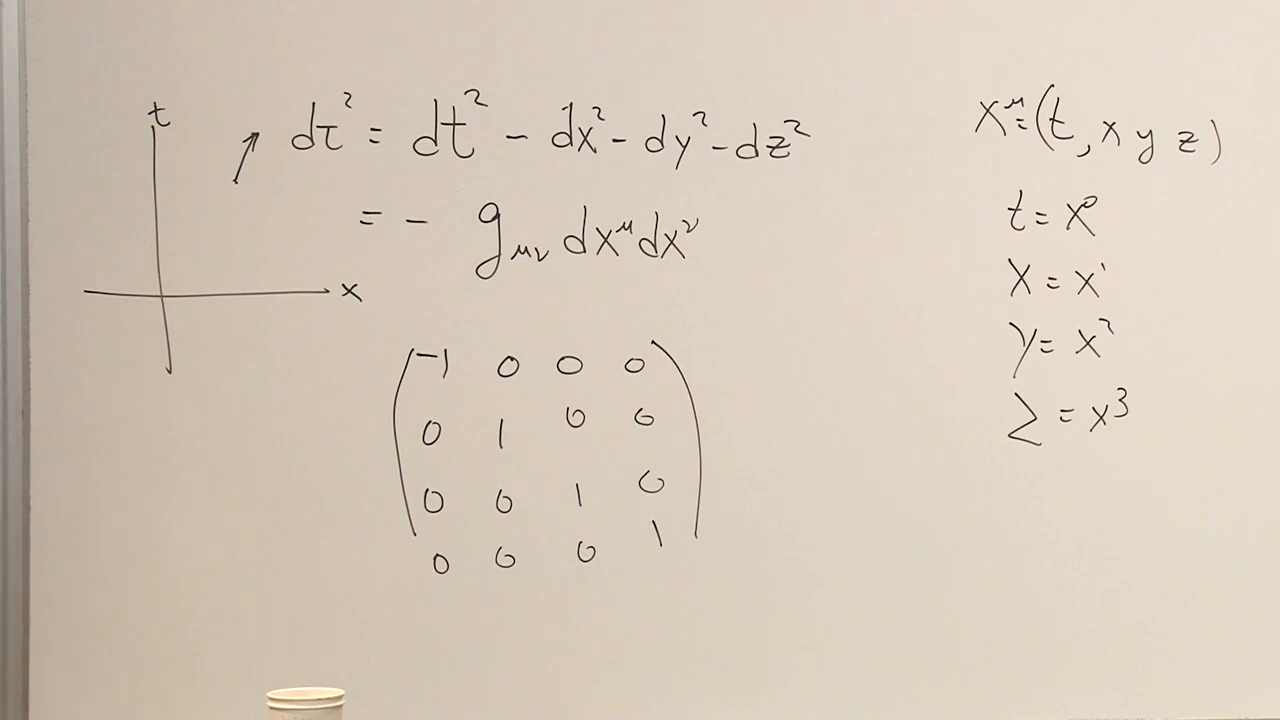
\includegraphics[width=0.92\textwidth]{lecture_04_figure_04.png}
\caption{Die gewöhnliche Komponentenänderung und die Korrektur durch die Verbindung entlang einer Kurve.}
\end{figure}

Der Vektor wird paralleltransportiert, wenn diese kovariante Änderung verschwindet:
\begin{equation}
\boxed{
dV^n+\Gamma^n{}_{mr}V^r\,dx^m=0.
}
\label{eq:l4-parallel-transport}
\end{equation}
Anschaulich können wir uns vorstellen, an jedem Punkt der Kurve ein Normalkoordinatensystem einzurichten. In diesem lokalen Bezugssystem darf sich der transportierte Vektor nicht drehen. Dann bewegen wir uns infinitesimal weiter, richten das nächste Normalkoordinatensystem ein und wiederholen den Vorgang.

\begin{figure}[htbp]
\centering
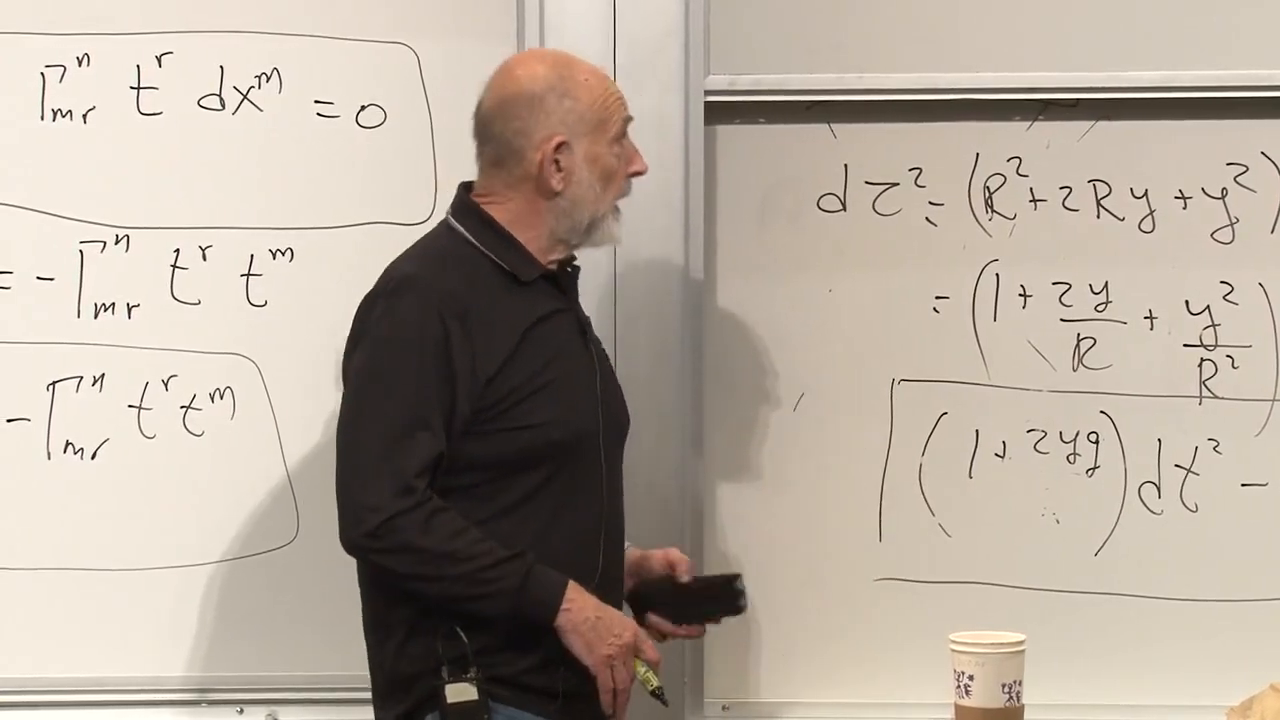
\includegraphics[width=0.92\textwidth]{lecture_04_figure_05.png}
\caption{Ein übersichtlicher Tafelstand der Paralleltransportgleichung.}
\end{figure}

Die Orientierung jedes vorübergehend verwendeten Normalkoordinatensystems gehört nicht zur Physik. Vor dem Vergleich könnten wir es drehen. Entscheidend ist, dass die kovariante Aussage \eqref{eq:l4-parallel-transport} unabhängig von dieser willkürlichen Wahl ist.

\subsection{Wegabhängigkeit und Krümmung}

In einem gekrümmten Raum hängt der Paralleltransport vom Weg ab. Wir beginnen mit demselben Vektor am selben Ausgangspunkt und transportieren ihn auf zwei verschiedenen Wegen zum selben Endpunkt. Im Allgemeinen unterscheiden sich die Endvektoren. Wird ein Vektor entlang einer geschlossenen Schleife mitgeführt, kann er gedreht zurückkehren. Diese Abweichung ist die Holonomie und ein unmittelbarer Hinweis auf Krümmung.

\begin{figure}[htbp]
\centering
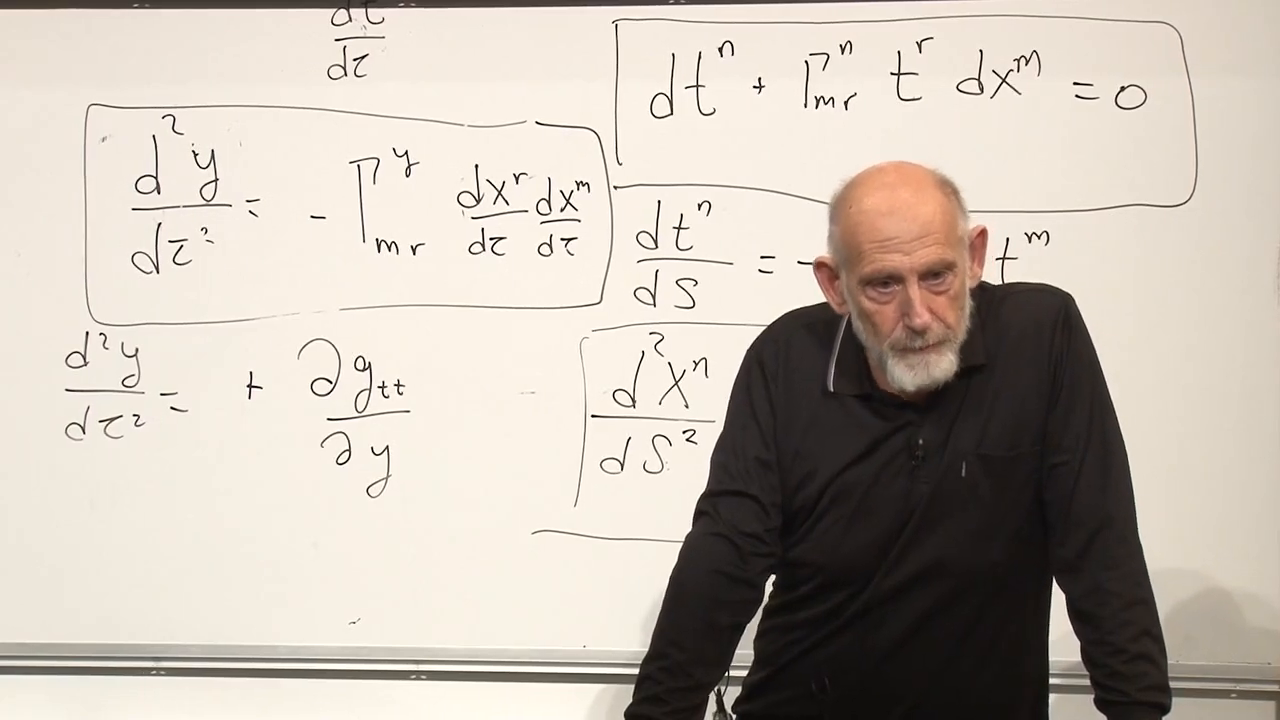
\includegraphics[width=0.90\textwidth]{lecture_04_figure_06.png}
\caption{Auf einer gekrümmten Fläche müssen zwei verschiedene Wege einen Vektor nicht in dieselbe Endorientierung transportieren.}
\end{figure}

Der Kegel ist ein anschauliches Beispiel. Abseits seiner Spitze kann man einen Kegel aufschneiden und flach ausbreiten. Beim Paralleltransport entlang einer Schleife, die die Spitze umschließt, kehrt der Vektor dennoch um den Winkel des Winkeld efekts gedreht zurück. Ist die Spitze abgerundet, ist die Krümmung endlich und über ein kleines Gebiet verteilt. Ist sie vollkommen scharf, konzentriert die Idealisierung die Krümmung an der Spitze.

\begin{figure}[htbp]
\centering
\includegraphics[width=0.90\textwidth]{lecture_04_figure_07.png}
\caption{Kreisbewegung auf dem Kegel und ihre aufgeschnittene ebene Darstellung.}
\end{figure}

\subsection{Fragen zum transportierten Vektor}

\paragraph{Muss der Vektor überall definiert sein?}
Nein. Man kann an einem einzelnen Punkt mit einem Vektor beginnen und \eqref{eq:l4-parallel-transport} nur entlang der gewählten Kurve lösen. Ein vollständiges Vektorfeld ist nicht erforderlich. Ist ein Feld auf einem Gebiet definiert, kann es entlang einer Richtung kovariant konstant sein, entlang einer anderen jedoch nicht.

\paragraph{Bleibt seine Länge erhalten?}
Ja. Sei \(V^2=g_{mn}V^mV^n\). Entlang der Kurve gilt
\begin{align}
\frac{D}{d\lambda}\left(g_{mn}V^mV^n\right)
&=
\frac{Dg_{mn}}{d\lambda}V^mV^n
+2g_{mn}V^m\frac{DV^n}{d\lambda}\\
&=0.
\end{align}
Die Metrikverträglichkeit lässt den ersten Term verschwinden, der Paralleltransport den zweiten. Längen und gegenseitige Winkel paralleltransportierter Vektoren bleiben daher erhalten.

\paragraph{Wird die Tangente an jede Kurve paralleltransportiert?}
Nein. Diese Frage führt unmittelbar zu den Geodäten. Die Tangente an einen Kreisweg um einen Kegel dreht sich fortwährend. Die Tangente an die gerade Linie, die nach dem Aufschneiden des Kegels entsteht, tut dies nicht. Nur der zweite Weg ist lokal gerade.

\section{Geodäten: möglichst gerade, nicht bloß möglichst kurz}

Eine Geodäte lässt sich auf zwei miteinander verwandte Weisen beschreiben. Global ist sie ein stationärer Weg für das Längen- oder Eigenzeitfunktional. Lokal ist sie der möglichst gerade Weg. Das Wort stationär ist wichtig: Je nach Geometrie und Endpunkten muss der Weg nicht das eindeutige globale Minimum sein. In der Lorentzschen Raumzeit maximieren zeitartige Geodäten lokal die Eigenzeit, statt eine positive Distanz zu minimieren.

Die lokale Beschreibung ist hier maßgeblich. Ein kleines Auto, das über gekrümmtes Gelände fährt und dessen Lenkrad unbeirrt geradeaus gehalten wird, beschreibt eine Geodäte, sofern das Auto klein gegenüber der Krümmungsskala des Geländes ist. In einem Einbettungsraum muss der Weg nicht gerade aussehen; gerade ist er gemäß der Geometrie, die auf der Fläche gilt.

\begin{figure}[htbp]
\centering
\includegraphics[width=0.90\textwidth]{lecture_04_figure_08.png}
\caption{Ein intrinsisch auf der gekrümmten Fläche eingezeichneter Weg als Vorbereitung auf die Definition des möglichst geraden Weges.}
\end{figure}

\subsection{Der Tangentialvektor}

Sei die Kurve \(x^m(s)\), mit der Bogenlänge
\begin{equation}
ds^2=g_{mn}\,dx^m dx^n.
\end{equation}
Der Einheitstangentialvektor ist
\begin{equation}
t^m=\frac{dx^m}{ds}.
\label{eq:l4-unit-tangent}
\end{equation}
Geometrisch nehmen wir zwei nahe Punkte, bilden den Verschiebungsvektor zwischen ihnen, teilen ihn durch ihren Abstand und lassen die Punkte zusammenrücken.

\begin{figure}[htbp]
\centering
\includegraphics[width=0.90\textwidth]{lecture_04_figure_09.png}
\caption{Die Tangentialrichtung als Grenzwert der Verschiebung entlang einer Kurve.}
\end{figure}

\begin{figure}[htbp]
\centering
\includegraphics[width=0.90\textwidth]{lecture_04_figure_10.png}
\caption{Das Linienelement und der Einheitstangentialvektor \(t^m=dx^m/ds\).}
\end{figure}

Eine Geodäte ist eine Kurve, deren Tangente entlang der Kurve selbst paralleltransportiert wird:
\begin{equation}
dt^n+\Gamma^n{}_{mr}t^r\,dx^m=0.
\end{equation}Teilen wir durch \(ds\) und verwenden \(dx^m/ds=t^m\):
\begin{equation}
\frac{dt^n}{ds}
=
-\Gamma^n{}_{mr}t^m t^r.
\end{equation}Setzen wir schließlich \(t^n=dx^n/ds\) ein:
\begin{equation}
\boxed{
\frac{d^2x^n}{ds^2}
+\Gamma^n{}_{mr}
\frac{dx^m}{ds}
\frac{dx^r}{ds}
=0.
}
\label{eq:l4-geodesic}
\end{equation}

\begin{figure}[htbp]
\centering
\includegraphics[width=0.94\textwidth]{lecture_04_figure_11.png}
\caption{Das Transportgesetz für den Tangentialvektor und die Geodätengleichung zweiter Ordnung.}
\end{figure}

Gleichung \eqref{eq:l4-geodesic} ähnelt bereits der Newtonschen Dynamik. Ersetzen wir \(s\) durch einen geeigneten Zeitparameter, ist der erste Term eine Beschleunigung. Der Verbindungsterm wirkt dann wie eine Kraft pro Masseneinheit, die vollständig durch die Metrik bestimmt ist. In der allgemeinen Relativitätstheorie wird diese Analogie wörtlich: Freie Teilchen folgen Geodäten der Raumzeit, und das, was Newton Gravitationsbeschleunigung nannte, tritt über die Verbindung in Erscheinung.

\section{Von der Riemannschen Distanz zur Eigenzeit in der Raumzeit}

Nun geht die Betrachtung vom gekrümmten Raum zur Raumzeit über. In inertialen kartesischen Koordinaten lautet die Eigenzeit zwischen benachbarten Ereignissen
\begin{equation}
d\tau^2
=dt^2-dx^2-dy^2-dz^2.
\label{eq:l4-proper-time}
\end{equation}
Die Vorlesung verwendet
\begin{equation}
d\tau^2=-g_{\mu\nu}\,dx^\mu dx^\nu
\label{eq:l4-lecture-sign}
\end{equation}
mit
\begin{equation}
g_{\mu\nu}
=
\eta_{\mu\nu}
=
\begin{pmatrix}
-1&0&0&0\\
0&1&0&0\\
0&0&1&0\\
0&0&0&1
\end{pmatrix}.
\label{eq:l4-eta}
\end{equation}
Das äußere Minuszeichen in \eqref{eq:l4-lecture-sign} überführt also die gewählte Metrik mit überwiegend positiven Vorzeichen in \eqref{eq:l4-proper-time}. Die Koordinaten sind
\begin{equation}
\begin{aligned}
x^\mu&=(t,x,y,z),\\
x^0&=t,\quad x^1=x,\\
x^2&=y,\quad x^3=z.
\end{aligned}
\end{equation}

\begin{figure}[htbp]
\centering
\includegraphics[width=0.94\textwidth]{lecture_04_figure_12.png}
\caption{Eigenzeit, Raumzeitkoordinaten und die Minkowski-Metrik mit überwiegend positiven Vorzeichen.}
\end{figure}

Die Signatur ist die invariante Information: Ein Eigenwert hat das Vorzeichen der Zeitrichtung, drei haben das Vorzeichen der Raumrichtungen. Multipliziert man die gesamte Metrik mit \(-1\) und passt alle Konventionen konsistent an, erhält man die ebenso verbreitete Konvention mit überwiegend negativen Vorzeichen. Von dieser Gesamtwahl hängt keine physikalische Aussage ab.

In der Vorlesung wird gefragt, ob Räume mit anderen indefiniten Signaturen betrachtet wurden. Mathematisch sind pseudo-riemannsche Geometrien mit vielen verschiedenen Signaturen gut etabliert. Der physikalische Punkt ist enger gefasst: Die beobachtete relativistische Raumzeit ist Lorentzsch, mit einer zeitartigen Richtung. Weitere zeitartige Richtungen würden die Kausalstruktur tiefgreifend verändern und beschreiben nicht die hier behandelte Physik.

\begin{figure}[htbp]
\centering
\includegraphics[width=0.94\textwidth]{lecture_04_figure_13.png}
\caption{Vor der Bezeichnung der flachen Metrik mit \(\eta_{\mu\nu}\) wird die Vorzeichenkonvention überprüft.}
\end{figure}

Dass die Raumzeit flach ist, bedeutet nicht, dass die Metrikkomponenten in jedem Koordinatensystem wie \(\eta_{\mu\nu}\) aussehen müssen. Es bedeutet, dass Koordinaten existieren, in denen sie diese Form haben. In krummlinigen oder beschleunigten Koordinaten können sich die Komponenten mit dem Ort ändern, obwohl der Riemann-Tensor null ist.

\section{Warum gleiche Koordinatenbeschleunigung nicht starr ist}

Wir suchen Koordinaten, die an einen beschleunigten Aufzug gebunden sind. Der erste Gedanke ist, eine Reihe von Beobachtern in festen Abständen aufzustellen und ihnen allen dieselbe Koordinatenbeschleunigung zu geben. Die Relativitätstheorie verhindert, dass diese naive Konstruktion starr bleibt.

\begin{figure}[htbp]
\centering
\includegraphics[width=0.92\textwidth]{lecture_04_figure_14.png}
\caption{Eine Reihe benachbarter Beobachter zur Prüfung, ob eine gemeinsame Beschleunigung die Starrheit erhält.}
\end{figure}

Folgen getrennte Beobachter nach einem einzigen Inertialsystem identischen Beschleunigungsabläufen, bleibt ihr Abstand in den sich ändernden momentanen Ruhesystemen nicht konstant. Eine sie verbindende Schnur wird gedehnt und reißt schließlich. Das ist dieselbe kinematische Spannung wie im Gedankenexperiment mit Bells Raumschiffen. Außerdem kann eine konstante Newtonsche Koordinatenbeschleunigung nicht unbegrenzt andauern: Sie würde schließlich eine Geschwindigkeit oberhalb der Lichtgeschwindigkeit vorhersagen.

Ein relativistisch starr beschleunigtes Bezugssystem muss daher an jedem Ort eine andere Eigenbeschleunigung aufweisen. Die Beobachter in der Nähe des hypothetischen Horizonts beschleunigen stärker, die weiter entfernten schwächer. Dadurch können ihre Eigenabstände im momentanen mitbewegten Bezugssystem konstant bleiben. Dies ist Bornsche Starrheit bei einer Dimension des Raums.

\section{Euklidische Polarkoordinaten als Vorbereitung}

Die richtige Konstruktion lässt sich am einfachsten anhand eines gewöhnlichen Kreises erkennen. In einer euklidischen Ebene gilt
\begin{equation}
x=r\cos\theta,
\qquad
y=r\sin\theta,
\end{equation}
also
\begin{equation}
x^2+y^2=r^2,
\qquad
\cos^2\theta+\sin^2\theta=1.
\end{equation}
Die Darstellungen mit komplexen Exponentialfunktionen lauten
\begin{equation}
\cos\theta=\frac{e^{i\theta}+e^{-i\theta}}{2},
\qquad
\sin\theta=\frac{e^{i\theta}-e^{-i\theta}}{2i}.
\label{eq:l4-euler-trig}
\end{equation}
Bei der Tafelbesprechung wird der Faktor \(i\) im Nenner der Sinusformel bemerkt und wieder eingesetzt.

\begin{figure}[htbp]
\centering
\includegraphics[width=0.94\textwidth]{lecture_04_figure_15.png}
\caption{Der Kreis, euklidische Polarkoordinaten und ihre Darstellung mithilfe hyperbolischer Funktionen.}
\end{figure}

Ein fester Wert von \(r\) beschreibt einen Kreis. Bei konstanter Winkelgeschwindigkeit ist der Betrag der Zentripetalbeschleunigung konstant; sie zeigt stets nach innen. In der Raumzeit übernimmt die Hyperbel die entsprechende Rolle.

\section{Hyperbolische Koordinaten in der Minkowski-Raumzeit}

Wir ersetzen die trigonometrischen Funktionen durch ihre hyperbolischen Verwandten:
\begin{equation}
\cosh\omega=\frac{e^\omega+e^{-\omega}}{2},
\qquad
\sinh\omega=\frac{e^\omega-e^{-\omega}}{2},
\end{equation}mit
\begin{equation}
\cosh^2\omega-\sinh^2\omega=1.
\label{eq:l4-hyperbolic-identity}
\end{equation}
Einen Faktor \(i\) gibt es hier nicht. Die Koordinate \(\omega\) ist ein hyperbolischer Winkel, also die Rapidität. Anders als ein gewöhnlicher Winkel ist sie nicht periodisch; sie reicht von \(-\infty\) bis \(+\infty\).

\begin{figure}[htbp]
\centering
\includegraphics[width=0.94\textwidth]{lecture_04_figure_16.png}
\caption{Bei der Konstruktion der Raumzeit treten hyperbolische Funktionen an die Stelle trigonometrischer Funktionen.}
\end{figure}

Wir definieren neue Koordinaten im rechten Rindler-Keil:
\begin{equation}
x=r\cosh\omega,
\qquad
t=r\sinh\omega,
\qquad
r>0.
\label{eq:l4-rindler-transform}
\end{equation}Dann gilt
\begin{equation}
x^2-t^2=r^2.
\label{eq:l4-rindler-hyperbola}
\end{equation}Bei festem \(r\) beschreibt eine Änderung von \(\omega\) eine Hyperbel. Eine Zunahme von \(r\) führt quer durch die Familie in eine raumartige Richtung, während eine Zunahme von \(\omega\) entlang einer Hyperbel in eine zeitartige Richtung führt.

\begin{figure}[htbp]
\centering
\includegraphics[width=0.94\textwidth]{lecture_04_figure_17.png}
\caption{Die Koordinatentransformation \(x=r\cosh\omega\), \(t=r\sinh\omega\) und ihre invariante Hyperbel.}
\end{figure}

\begin{figure}[htbp]
\centering
\includegraphics[width=0.94\textwidth]{lecture_04_figure_18.png}
\caption{Eine Kongruenz von Hyperbeln mit festem \(r\), die eine starr beschleunigte Familie darstellen.}
\end{figure}

\subsection{Die Metrik in beschleunigten Koordinaten}

Wir differenzieren \eqref{eq:l4-rindler-transform}:
\begin{align}
dx&=\cosh\omega\,dr+r\sinh\omega\,d\omega,\\
dt&=\sinh\omega\,dr+r\cosh\omega\,d\omega.
\end{align}Mit \eqref{eq:l4-hyperbolic-identity} heben sich die Kreuzterme auf:
\begin{align}
d\tau^2
&=dt^2-dx^2\\
&=r^2\,d\omega^2-dr^2.
\label{eq:l4-rindler-metric}
\end{align}
Ergänzt man die transversalen Richtungen, kommt einfach \(-dy^2-dz^2\) hinzu; dabei gilt die hier verwendete Eigenzeitkonvention.

Dies ist nach wie vor eine flache Raumzeit. Der ortsabhängige Koeffizient \(r^2\) ist ebenso wenig ein Hinweis auf Krümmung wie der Faktor \(r^2\) vor \(d\theta^2\) in euklidischen Polarkoordinaten.

\subsection{Eigenbeschleunigung entlang der Hyperbeln}

Für eine feste Weltlinie \(r=R\) liefert Gleichung \eqref{eq:l4-rindler-metric}
\begin{equation}
d\tau=R\,d\omega.
\end{equation}Ihre Vierergeschwindigkeit ist
\begin{equation}
U^\mu
=
\frac{d(t,x)}{d\tau}
=
(\cosh\omega,\sinh\omega),
\end{equation}und ihre Viererbeschleunigung
\begin{equation}
A^\mu
=
\frac{dU^\mu}{d\tau}
=
\frac{1}{R}(\sinh\omega,\cosh\omega).
\end{equation}Der invariante Betrag ist konstant:
\begin{equation}
a=\sqrt{A^\mu A_\mu}=\frac{1}{R}
\qquad (c=1).
\label{eq:l4-proper-acceleration}
\end{equation}

\begin{figure}[htbp]
\centering
\includegraphics[width=0.90\textwidth]{lecture_04_figure_19.png}
\caption{Das Gesetz des umgekehrten Radius \(a=1/R\) für eine festgelegte beschleunigte Weltlinie.}
\end{figure}

Mit wieder eingesetzten Einheiten gilt
\begin{equation}
\boxed{a=\frac{c^2}{R}.}
\label{eq:l4-proper-acceleration-units}
\end{equation}

\begin{figure}[htbp]
\centering
\includegraphics[width=0.90\textwidth]{lecture_04_figure_20.png}
\caption{Mit wieder eingesetzten Einheiten wird aus \(1/R\) der Ausdruck \(c^2/R\).}
\end{figure}

Je kleiner der Achsenabschnitt \(R\) ist, desto stärker krümmt sich die Weltlinie und desto größer ist die Eigenbeschleunigung, die ihr Beobachter erfährt. Weiter außen liegende Hyperbeln krümmen sich weniger und erfordern eine geringere Beschleunigung. Jeder Beobachter hat eine zeitlich konstante Beschleunigung, doch die Beschleunigungen der verschiedenen Beobachter unterscheiden sich. Genau diese Variation erhält ihre gegenseitigen Eigenabstände.

\subsection{Fragen zu den beschleunigten Koordinaten}

\paragraph{Ist \(R\) der \(x\)-Achsenabschnitt?}
Ja. Bei \(\omega=0\) ergeben sich aus Gleichung \eqref{eq:l4-rindler-transform} die Werte \(t=0\) und \(x=R\). Der Achsenabschnitt legt über \eqref{eq:l4-proper-acceleration-units} die Eigenbeschleunigung fest.

\paragraph{Hängt die Konstruktion vom gewählten Ursprung ab?}
Ja, die Koordinaten hängen davon ab. Eine Verschiebung des Ursprungs ergibt eine andere Hyperbelfamilie mit verschobenen Asymptoten. Keine invariante physikalische Aussage hängt von dieser Wahl ab. Wir wählen bewusst ein beschleunigtes Koordinatensystem aus und fragen, wie sich darin die Trägheitsbewegung darstellt.

\paragraph{Was ist Eigenbeschleunigung?}
Sie ist die Beschleunigung, die ein mit dem Beobachter mitgeführtes Beschleunigungsmessgerät misst. Kovariant gilt
\begin{equation}
A^\mu=\frac{dU^\mu}{d\tau},
\qquad
U^\mu=\frac{dx^\mu}{d\tau}.
\end{equation}Ihr Betrag ist der Schub, den der Beobachter tatsächlich spürt, und nicht die Koordinatenbeschleunigung \(d^2x/dt^2\), die ein entferntes Bezugssystem zuweist.

\section{Flache Metriken in polaren und hyperbolischen Koordinaten}

Bevor wir die Betrachtung auf die Umgebung der Erde beschränken, stellen wir zweckmäßig die euklidische und die Lorentzsche Metrik einander gegenüber. In der Ebene gilt
\begin{equation}
ds^2=dr^2+r^2d\theta^2,
\qquad
g_{ab}
=
\begin{pmatrix}
1&0\\
0&r^2
\end{pmatrix}.
\label{eq:l4-polar-metric}
\end{equation}
Ein Vorschlag aus dem Publikum bringt kurz einen sphärischen Faktor ins Spiel, doch es handelt sich hier nur um eine Ebene, nicht um eine Kugel. Der Term \(r^2\) hält fest, dass ein festes Winkelintervall bei größerem Radius einen längeren Kreisbogen umfasst.

\begin{figure}[htbp]
\centering
\includegraphics[width=0.94\textwidth]{lecture_04_figure_21.png}
\caption{Die euklidische Polarmetrik: ortsabhängige Komponenten in einer flachen Ebene.}
\end{figure}

Das Minkowski-Analogon lautet
\begin{equation}
d\tau^2=r^2d\omega^2-dr^2.
\end{equation}
Beide Metriken haben ortsabhängige Komponenten, obwohl beide Geometrien flach sind. Koordinatenkrümmung und geometrische Krümmung sind nicht dasselbe.

\section{Lokale Betrachtung der erdnahen Beschleunigung}

Wir wählen eine Referenzhyperbel mit der Eigenbeschleunigung des Erdfeldes \(g\):
\begin{equation}
g=\frac{c^2}{R},
\qquad
R=\frac{c^2}{g}.
\label{eq:l4-earth-radius}
\end{equation}

\begin{figure}[htbp]
\centering
\includegraphics[width=0.94\textwidth]{lecture_04_figure_22.png}
\caption{Auswahl der Referenzhyperbel durch \(c^2/R=g\).}
\end{figure}

Numerisch gilt
\begin{equation}
R
\simeq
\frac{(3.0\times10^8\ {\rm m\,s^{-1}})^2}
{9.8\ {\rm m\,s^{-2}}}
\simeq
9.2\times10^{15}\ {\rm m}.
\end{equation}
Die Vorlesung rundet dies auf \(10^{16}\) Meter. Ein Feld von einer irdischen \(g\) ist auf relativistischen Skalen moderat; deshalb ist der zugehörige Rindler-Radius enorm.

Nun betrachten wir nur eine kleine Umgebung dieses Referenzbeobachters. Wir führen eine lokale Höhenkoordinate \(y\) ein durch
\begin{equation}
r=R+y,
\qquad
dr=dy,
\qquad
|y|\ll R.
\label{eq:l4-local-height}
\end{equation}
Die Gleichheit \(dr=dy\) wird in der Besprechung ausdrücklich bemerkt; daher muss der räumliche Term als \(-dy^2\) geschrieben werden.

Einsetzen in \eqref{eq:l4-rindler-metric} ergibt
\begin{align}
d\tau^2
&=(R+y)^2d\omega^2-dy^2\\
&=(R^2+2Ry+y^2)d\omega^2-dy^2\\
&=
\left(
1+\frac{2y}{R}+\frac{y^2}{R^2}
\right)
R^2d\omega^2-dy^2.
\label{eq:l4-local-expand}
\end{align}

\begin{figure}[htbp]
\centering
\includegraphics[width=0.94\textwidth]{lecture_04_figure_23.png}
\caption{Entwicklung der beschleunigten Metrik um \(r=R+y\).}
\end{figure}

Wir definieren eine lokale Zeitkoordinate
\begin{equation}
t=R\omega.
\label{eq:l4-local-time}
\end{equation}Dann gilt
\begin{equation}
d\tau^2
=
\left(
1+\frac{2y}{R}+\frac{y^2}{R^2}
\right)dt^2-dy^2.
\label{eq:l4-local-exact}
\end{equation}

\begin{figure}[htbp]
\centering
\includegraphics[width=0.94\textwidth]{lecture_04_figure_24.png}
\caption{Einführung von \(t=R\omega\) nach der Entwicklung um die Referenzhyperbel.}
\end{figure}

Selbst eine vertikale Strecke von mehreren zehn Kilometern ist klein gegenüber \(R\). Die Vorlesung veranschaulicht den Vergleich anhand eines Falls von ungefähr 24 Meilen: Selbst diese Strecke ist gegenüber \(10^{16}\) Metern vernachlässigbar. Daher ist \(y^2/R^2\) viel kleiner als \(y/R\), und der quadratische Term kann weggelassen werden:
\begin{equation}
d\tau^2
\simeq
\left(1+\frac{2y}{R}\right)dt^2-dy^2.
\label{eq:l4-local-linear}
\end{equation}

\begin{figure}[htbp]
\centering
\includegraphics[width=0.94\textwidth]{lecture_04_figure_25.png}
\caption{Die entwickelte Metrik und die Substitution der lokalen Zeit vor der Näherung für das schwache Feld.}
\end{figure}

In Einheiten mit \(c=1\) ergibt sich aus Gleichung \eqref{eq:l4-earth-radius} die Beziehung \(1/R=g\) und damit
\begin{equation}
\boxed{
d\tau^2\simeq(1+2gy)\,dt^2-dy^2.
}
\label{eq:l4-uniform-metric}
\end{equation}

\begin{figure}[htbp]
\centering
\includegraphics[width=0.94\textwidth]{lecture_04_figure_26.png}
\caption{Die vollständige lokale Metrik für den gleichförmig beschleunigten Aufzug.}
\end{figure}

Die Größe
\begin{equation}
\Phi(y)=gy
\end{equation}
ist das Newtonsche Gravitationspotential pro Masseneinheit in einem gleichförmigen Feld. Somit gilt
\begin{equation}
d\tau^2\simeq(1+2\Phi)\,dt^2-dy^2
\qquad (c=1).
\label{eq:l4-weak-potential-propertime}
\end{equation}
Mit der Konvention der Vorlesung \(d\tau^2=-g_{\mu\nu}dx^\mu dx^\nu\) bedeutet dies
\begin{equation}
g_{tt}=-(1+2\Phi).
\label{eq:l4-gtt-potential}
\end{equation}
In herkömmlichen Einheiten lautet die dimensionslose Korrektur \(2\Phi/c^2\).

Die Raumzeit ist nicht gekrümmt worden. Gleichung \eqref{eq:l4-uniform-metric} ist die lokale Entwicklung einer flachen Rindler-Metrik. Die scheinbare Gravitation entspricht der Trägheitskraft, die im Inneren eines beschleunigten Aufzugs wahrgenommen wird.

\section{Die Geodätengleichung wird zum Newtonschen Gesetz}

Die Identifizierung von \(gy\) mit einem Potential war bislang nur ein Hinweis. Die entscheidende Prüfung ist dynamischer Art: Beschleunigt ein freies Teilchen in der Metrik \eqref{eq:l4-uniform-metric} nach unten mit \(d^2y/dt^2=-g\)?

Für eine zeitartige Weltlinie, parametrisiert durch die Eigenzeit, gilt
\begin{equation}
\frac{d^2x^\nu}{d\tau^2}
+\Gamma^\nu{}_{\mu\rho}
\frac{dx^\mu}{d\tau}
\frac{dx^\rho}{d\tau}
=0.
\label{eq:l4-spacetime-geodesic}
\end{equation}
Die vertikale Komponente lautet
\begin{equation}
\frac{d^2y}{d\tau^2}
=
-\Gamma^y{}_{\mu\rho}
\frac{dx^\mu}{d\tau}
\frac{dx^\rho}{d\tau}.
\label{eq:l4-y-geodesic}
\end{equation}

\begin{figure}[htbp]
\centering
\includegraphics[width=0.94\textwidth]{lecture_04_figure_27.png}
\caption{Die Transportgleichung und ihre Geodätenform zweiter Ordnung, bereit zur Anwendung auf die vertikale Bewegung.}
\end{figure}

\subsection{Die Näherung für kleine Geschwindigkeiten}

Für ein langsam bewegtes Teilchen in einem schwachen, statischen Feld gilt
\begin{equation}
\frac{dt}{d\tau}\simeq1,
\qquad
\left|\frac{dy}{d\tau}\right|\ll1.
\end{equation}
Die Zeitkomponente der Vierergeschwindigkeit ist daher von der Größenordnung eins, während die räumlichen Komponenten im Vergleich dazu klein sind. Unter den Produkten in \eqref{eq:l4-y-geodesic} ist der Beitrag mit \(\mu=\rho=t\) der größte:
\begin{equation}
\frac{d^2y}{d\tau^2}
\simeq
-\Gamma^y{}_{tt}
\left(\frac{dt}{d\tau}\right)^2
\simeq
-\Gamma^y{}_{tt}.
\label{eq:l4-slow-geodesic}
\end{equation}

\begin{figure}[htbp]
\centering
\includegraphics[width=0.94\textwidth]{lecture_04_figure_28.png}
\caption{Spezialisierung der Geodätengleichung der Raumzeit auf die \(y\)-Komponente für kleine Geschwindigkeiten.}
\end{figure}

Nun berechnen wir den einen benötigten Verbindungkoeffizienten. Die Metrik ist diagonal und unabhängig von \(t\), daher gilt
\begin{align}
\Gamma^y{}_{tt}
&=
\frac{1}{2}g^{yy}
\left(
\partial_tg_{yt}
+\partial_tg_{ty}
-\partial_yg_{tt}
\right)\\
&=
-\frac{1}{2}\partial_yg_{tt},
\label{eq:l4-gamma-ytt}
\end{align}denn in der Vorzeichenkonvention der Vorlesung für den metrischen Tensor ist \(g^{yy}=1\).

\begin{figure}[htbp]
\centering
\includegraphics[width=0.94\textwidth]{lecture_04_figure_29.png}
\caption{Die Christoffel-Formel, spezialisiert auf die Komponente \(y,t,t\).}
\end{figure}

Zusammen mit \eqref{eq:l4-slow-geodesic} und \eqref{eq:l4-gamma-ytt} erhalten wir
\begin{equation}
\frac{d^2y}{d\tau^2}
\simeq
\frac{1}{2}\partial_yg_{tt}.
\label{eq:l4-accel-gtt}
\end{equation}Aus \eqref{eq:l4-gtt-potential} folgt
\begin{equation}
\partial_yg_{tt}
=
-2\partial_y\Phi
=
-2g.
\end{equation}Damit ergibt sich
\begin{equation}
\boxed{
\frac{d^2y}{d\tau^2}=-g.
}
\label{eq:l4-newton-result}
\end{equation}Da in derselben Näherung für kleine Geschwindigkeiten \(t\simeq\tau\) gilt, lautet das Ergebnis auch
\begin{equation}
\frac{d^2y}{dt^2}=-g.
\end{equation}

\begin{figure}[htbp]
\centering
\includegraphics[width=0.94\textwidth]{lecture_04_figure_30.png}
\caption{Die vollständige Vorzeichenkette: Die Ableitung von \(y\) nach \(g_{tt}\) ergibt die Beschleunigung \(-g\).}
\end{figure}

Allgemeiner gilt im Newtonschen Grenzfall
\begin{equation}
\boxed{
\begin{aligned}
g_{tt}&=-(1+2\Phi),\\
\frac{d^2x^i}{dt^2}&=-\partial_i\Phi
\end{aligned}
}
\qquad(c=1).
\label{eq:l4-newton-general}
\end{equation}
Mit wieder eingesetzten Einheiten lautet die metrische Korrektur \(2\Phi/c^2\), während die Beschleunigung \(-\boldsymbol{\nabla}\Phi\) bleibt.

Diese Rechnung erklärt, warum die Metrik und nicht ein gesondertes Gravitationskraftfeld das zentrale Objekt ist. Ein freies Teilchen folgt einfach einer Geodäte der Raumzeit. In Koordinaten, die an ein beschleunigtes Labor angepasst sind, weist diese Geodäte die Koordinatenkrümmung auf, die gewöhnlich der Gravitation zugeschrieben wird.

\subsection{Eine Frage zum gewählten Rindler-Ursprung}

Könnte die Referenzhyperbel so verschoben werden, dass ihre Asymptoten und ihr Achsenabschnitt an anderer Stelle liegen? Ja. Zu jedem geeignet verschobenen Ursprung gehört ein gleichförmig beschleunigtes Koordinatensystem. Im Bild des Aufzugs entspricht dies der Wahl von Aufzügen, deren Böden sich zu einem bestimmten Zeitpunkt an verschiedenen Orten befinden.

Das lokale Ergebnis hängt nicht von einem ausgezeichneten Ursprung ab. Nachdem ein Referenzbeobachter mit Beschleunigung \(g\) ausgewählt wurde, misst \(y\) die Höhe relativ zu diesem Beobachter, und die nahe Metrik hat die Form \eqref{eq:l4-uniform-metric}. Die willkürliche Koordinatenwahl bestimmt, wo wir den Boden beschreiben; sie erzeugt keine invariante Krümmung.

\section{Warum das Christoffel-Symbol kein Tensor sein darf}

Die Diskussion nach der Vorlesung greift einen Punkt wieder auf, der bereits in der Wiederholung zur Sprache kam. In den ursprünglichen Inertialkoordinaten gilt
\begin{equation}
g_{\mu\nu}=\eta_{\mu\nu},
\qquad
\partial_\rho\eta_{\mu\nu}=0,
\qquad
\Gamma^\mu{}_{\nu\rho}=0.
\end{equation}
Ein freies Teilchen bewegt sich geradlinig, und es gibt keine Gravitationskraft.

In den beschleunigten Koordinaten hat dieselbe flache Raumzeit ortsabhängige Metrikkomponenten. Ihre Christoffel-Symbole verschwinden nicht, und dieselbe Trägheitsbahn erscheint gekrümmt. Das Teilchen scheint zum Boden des Aufzugs zu fallen.

Das wäre unmöglich, wenn \(\Gamma^\mu{}_{\nu\rho}\) ein Tensor wäre. Ein Tensor, der in einem Bezugssystem verschwindet, verschwindet in jedem Bezugssystem. Die Verbindung erhält bei einer Koordinatentransformation stattdessen einen inhomogenen Term; daher kann sie in einem Inertialsystem null und in einem beschleunigten System ungleich null sein. Genau dies verlangt das Äquivalenzprinzip:
\begin{equation}
\text{accelerated frame}
\quad\longleftrightarrow\quad
\text{local gravity}.
\end{equation}

Die Krümmung verhält sich anders. Der Riemann-Tensor ist ein Tensor. Verschwindet er im Inertialsystem, so verschwindet er auch im beschleunigten System:
\begin{equation}
R^\mu{}_{\nu\rho\sigma}=0.
\end{equation}
Die Christoffel-Symbole beschreiben somit eine koordinatenabhängige Gravitationskraft, während die Krümmung den invarianten Gezeitenanteil erfasst, den keine Koordinatentransformation beseitigen kann.

\section{Vom gleichförmigen Potential zur Vorschau auf Schwarzschild}

Im beschleunigten Aufzug gibt es weder gravitative Materie noch Krümmung. Dennoch legt die Schwachfeldbeziehung \eqref{eq:l4-newton-general} nahe, wonach wir im Feld einer tatsächlich vorhandenen Kugelmasse suchen sollten. Das Newtonsche Potential außerhalb einer Masse \(M\) lautet
\begin{equation}
\Phi(r)=-\frac{GM}{r}.
\label{eq:l4-newton-potential}
\end{equation}
Setzen wir es in die Zeitkomponente des schwachen Feldes ein, erhalten wir
\begin{equation}
g_{tt}
\simeq
-\left(1-\frac{2GM}{r}\right)
\qquad(c=1).
\label{eq:l4-schwarzschild-preview}
\end{equation}
Das Vorzeichen des Potentials wird bei der Tafelbesprechung korrigiert. Anziehung erfordert ein negatives Potential, das sich von unten null nähert, wenn \(r\) gegen unendlich geht.

\begin{figure}[htbp]
\centering
\includegraphics[width=0.94\textwidth]{lecture_04_figure_31.png}
\caption{Das Newtonsche Potential eingesetzt in den Zeit-Zeit-Koeffizienten der Metrik; so zeigt sich der Faktor \(1-2GM/r\).}
\end{figure}

Der Koeffizient verschwindet bei
\begin{equation}
r=2GM
\qquad(c=1),
\end{equation}
oder, mit wieder eingesetzten Einheiten,
\begin{equation}
r_s=\frac{2GM}{c^2}.
\end{equation}
Dies ist der Schwarzschild-Radius. Das Verschwinden dieses speziellen Metrikkoeffizienten deutet einen Horizont an.

Das Argument wird bewusst als Vorschau und nicht als Herleitung präsentiert. Die Schwachfeldnäherung allein kann die exakte Schwarzschild-Lösung in der Nähe von \(r=2GM/c^2\) nicht begründen, genau dort, wo die Korrektur nicht mehr klein ist. Die vollständige Lösung enthält außerdem eine nichttriviale radiale Komponente und muss Einsteins Feldgleichungen erfüllen. Diese Gleichungen wurden noch nicht eingeführt. Die vorliegende Argumentation gibt jedoch den richtigen strukturellen Hinweis und zeigt die Größenordnung, bei der etwas qualitativ Neues auftreten muss.

\section{Fragen und Korrekturen aus der Vorlesung}

\subsection{Verhält sich ein hyperbolischer Winkel wie ein gewöhnlicher Winkel?}

Nein. Beide parametrisieren die Bewegung entlang einer Familie von Kurven mit konstantem Radius, aber \(\theta\) ist periodisch, während die Rapidität \(\omega\) die gesamte reelle Gerade durchläuft. Das Wort Winkel bezeichnet die algebraische Analogie zwischen Drehungen und Lorentz-Boosts, nicht eine Größe, die auf den Bereich zwischen \(0\) und \(2\pi\) beschränkt ist.

\subsection{Warum erfordert eine mäßige Beschleunigung ein riesiges R?}

Die Beziehung \(a=c^2/R\) enthält die große relativistische Skala \(c^2\). Um lediglich \(10\ {\rm m\,s^{-2}}\) zu erhalten, muss \(R\) in der Größenordnung von \(10^{16}\) Metern liegen. Dabei handelt es sich nicht um eine neue physikalische Entfernung, die der Erde zugeordnet ist. Es ist der Krümmungsradius der hyperbolischen Weltlinie in einem Minkowski-Diagramm, ausgedrückt in Längeneinheiten.

Der große Radius gewährleistet außerdem ein brauchbares Newtonsches Zeitintervall. Bei Laborzeiten und -abständen bleibt die Geschwindigkeit weit unter \(c\), die Beschleunigung ändert sich über den Aufbau hinweg nur vernachlässigbar, und \(t\) unterscheidet sich nur wenig von der Eigenzeit.

\subsection{Ist das scheinbare Gravitationsfeld real?}

Für einen Beobachter, der an einer festen Rindler-Position gehalten wird, ist es als Anzeige eines Beschleunigungsmessers real; es entspricht jedoch keiner invarianten Krümmung. Gibt man den Beobachter frei, zeigt der Beschleunigungsmesser entlang der resultierenden inertialen Geodäte null an. Ein hinreichend kleines frei fallendes Labor kann das gleichförmige Feld lokal beseitigen. Über einen endlichen Bereich hinweg lässt sich ein Gezeitenfeld, das durch eine von null verschiedene Krümmung beschrieben wird, jedoch nicht beseitigen.

\subsection{Was wurde bei der Kraftberechnung korrigiert?}

Mehrere Vorzeichen und ein Faktor von einer Hälfte werden direkt überprüft. Die verlässliche Rechnungskette gemäß der in der Vorlesung verwendeten Konvention lautet
\begin{equation}
\begin{aligned}
g_{tt}&=-(1+2gy),\\
\Gamma^y{}_{tt}&=-\frac12\partial_yg_{tt}=g,\\
\frac{d^2y}{d\tau^2}&=-\Gamma^y{}_{tt}=-g.
\end{aligned}
\end{equation}
Wenn die Konvention ausdrücklich angegeben wird, kann ein kurzes Zögern wegen eines Vorzeichens an der Tafel nicht zu einer physikalischen Mehrdeutigkeit führen.

\section{Was wurde gezeigt}

Die Vorlesung beginnt mit Differentialgeometrie und endet bei Newtons fallendem Körper. Die wesentlichen Schritte sind:
\begin{enumerate}
\item Eine kovariante Ableitung vergleicht Tensoren in sich ändernden Koordinatenbasen.
\item Paralleltransport bedeutet, dass sich ein Tensor entlang eines gewählten Weges kovariant nicht ändert.
\item Bei einer Geodäte wird ihr eigener Tangentialvektor paralleltransportiert.
\item Freie Teilchen bewegen sich auf Geodäten der Raumzeit.
\item Hyperbeln mit festem \(r\) bilden ein relativistisch starres beschleunigtes Bezugssystem.
\item Ihre Eigenbeschleunigung beträgt \(a=c^2/r\) und muss daher mit der Position variieren.
\item In der Nähe einer Referenzweltlinie mit der Beschleunigung \(g\) lautet die flache Metrik:
\begin{equation}
d\tau^2\simeq(1+2gy)\,dt^2-dy^2
\qquad(c=1).
\end{equation}
\item Ihre Geodätengleichung reduziert sich auf
\begin{equation}
\frac{d^2y}{dt^2}=-g.
\end{equation}
\end{enumerate}

Das Äquivalenzprinzip ist daher nicht bloß eine Analogie zwischen einem Aufzug und der Gravitation. Es ist darin verankert, wie sich die Metrik und ihre Verbindung transformieren. Eine gleichförmige Gravitationskraft kann auftreten, wenn die flache Raumzeit in beschleunigten Koordinaten beschrieben wird, während die Krümmung null bleibt.

Die abschließende Extrapolation führt über das gleichförmige Feld hinaus. Ersetzt man \(\Phi=gy\) durch \(\Phi=-GM/r\), sagt dies den charakteristischen Faktor \(1-2GM/r\) in der Zeitkomponente einer sphärischen Metrik voraus und macht die Schwarzschild-Skala sichtbar. Um jedoch die vollständige Geometrie zu bestimmen, brauchen wir die Feldgleichungen. Mit dieser Aufgabe befasst sich die nächste Vorlesung.
